\subsection{Código MATLAB para dimensionamiento de $R_s$ y $R_c$}

%\addcontentsline{toc}{section}{Apéndice A. Código MATLAB}

\begin{lstlisting}[caption={Cálculo de resistencias Shunt $R_s$ y de calibración $R_c$ para un amperímetro de bobina móvil de tres rangos},label={lst:matlab_voltimetro}]
syms Rc Ig
s = 700; Rg = 391;
Rango1 = 10e-3; Rango2 = 50e-3; Rango3 = 100e-3;
Isen = 1/s;

Rsh1 = Rg * Isen/(Rango1-Isen);
Rsh2 = Rg * Isen/(Rango2-Isen);
Rsh3 = Rg * Isen/(Rango3-Isen);

I1 = @(Ig) Ig * (1+(Rc+Rg)/Rsh1);
I2 = @(Ig) Ig * (1+(Rc+Rg)/Rsh2);
I3 = @(Ig) Ig * (1+(Rc+Rg)/Rsh3);

expr = I1(1e-3); %Cuando mide la corriente maxima, está midiendo la corrinte de rango 1
eq = expr == Rango1; a = vpasolve(eq, Rc);
disp("El valor para rango 1 de Rc es: " + string(a));
eq = expr == Rango1*1.1; a = vpasolve(eq, Rc);
disp("Para +10%: " + string(a));
eq = expr == Rango1*0.9;
a = vpasolve(eq, Rc);
disp("Para -10%: " + string(a));
disp("Y el de Rsh: " + string(Rsh1));

expr = I2(1e-3); %Cuando mide la corriente maxima, está midiendo la corrinte de rango 2
eq = expr == Rango2; a = vpasolve(eq, Rc);
disp("El valor para rango 2 de Rc es: " + string(a));
eq = expr == Rango2*1.1; a = vpasolve(eq, Rc);
disp("Para +10%: " + string(a));
eq = expr == Rango2*0.9; a = vpasolve(eq, Rc);
disp("Para -10%: " + string(a));
disp("Y el de Rsh: " + string(Rsh2));

expr = I3(1e-3); %Cuando mide la corriente maxima, está midiendo la corrinte de rango 3
eq = expr == Rango3; a = vpasolve(eq, Rc);
disp("El valor para rango 3 de Rc es: " + string(a));
eq = expr == Rango3*1.1; a = vpasolve(eq, Rc);
disp("Para +10%: " + string(a));
eq = expr == Rango3*0.9; a = vpasolve(eq, Rc);
disp("Para -10%: " + string(a));
disp("Y el de Rsh: " + string(Rsh3));
\end{lstlisting}



\subsection{Imágenes cuaderno de preinforme}

\begin{figure}[H]
    \centering
    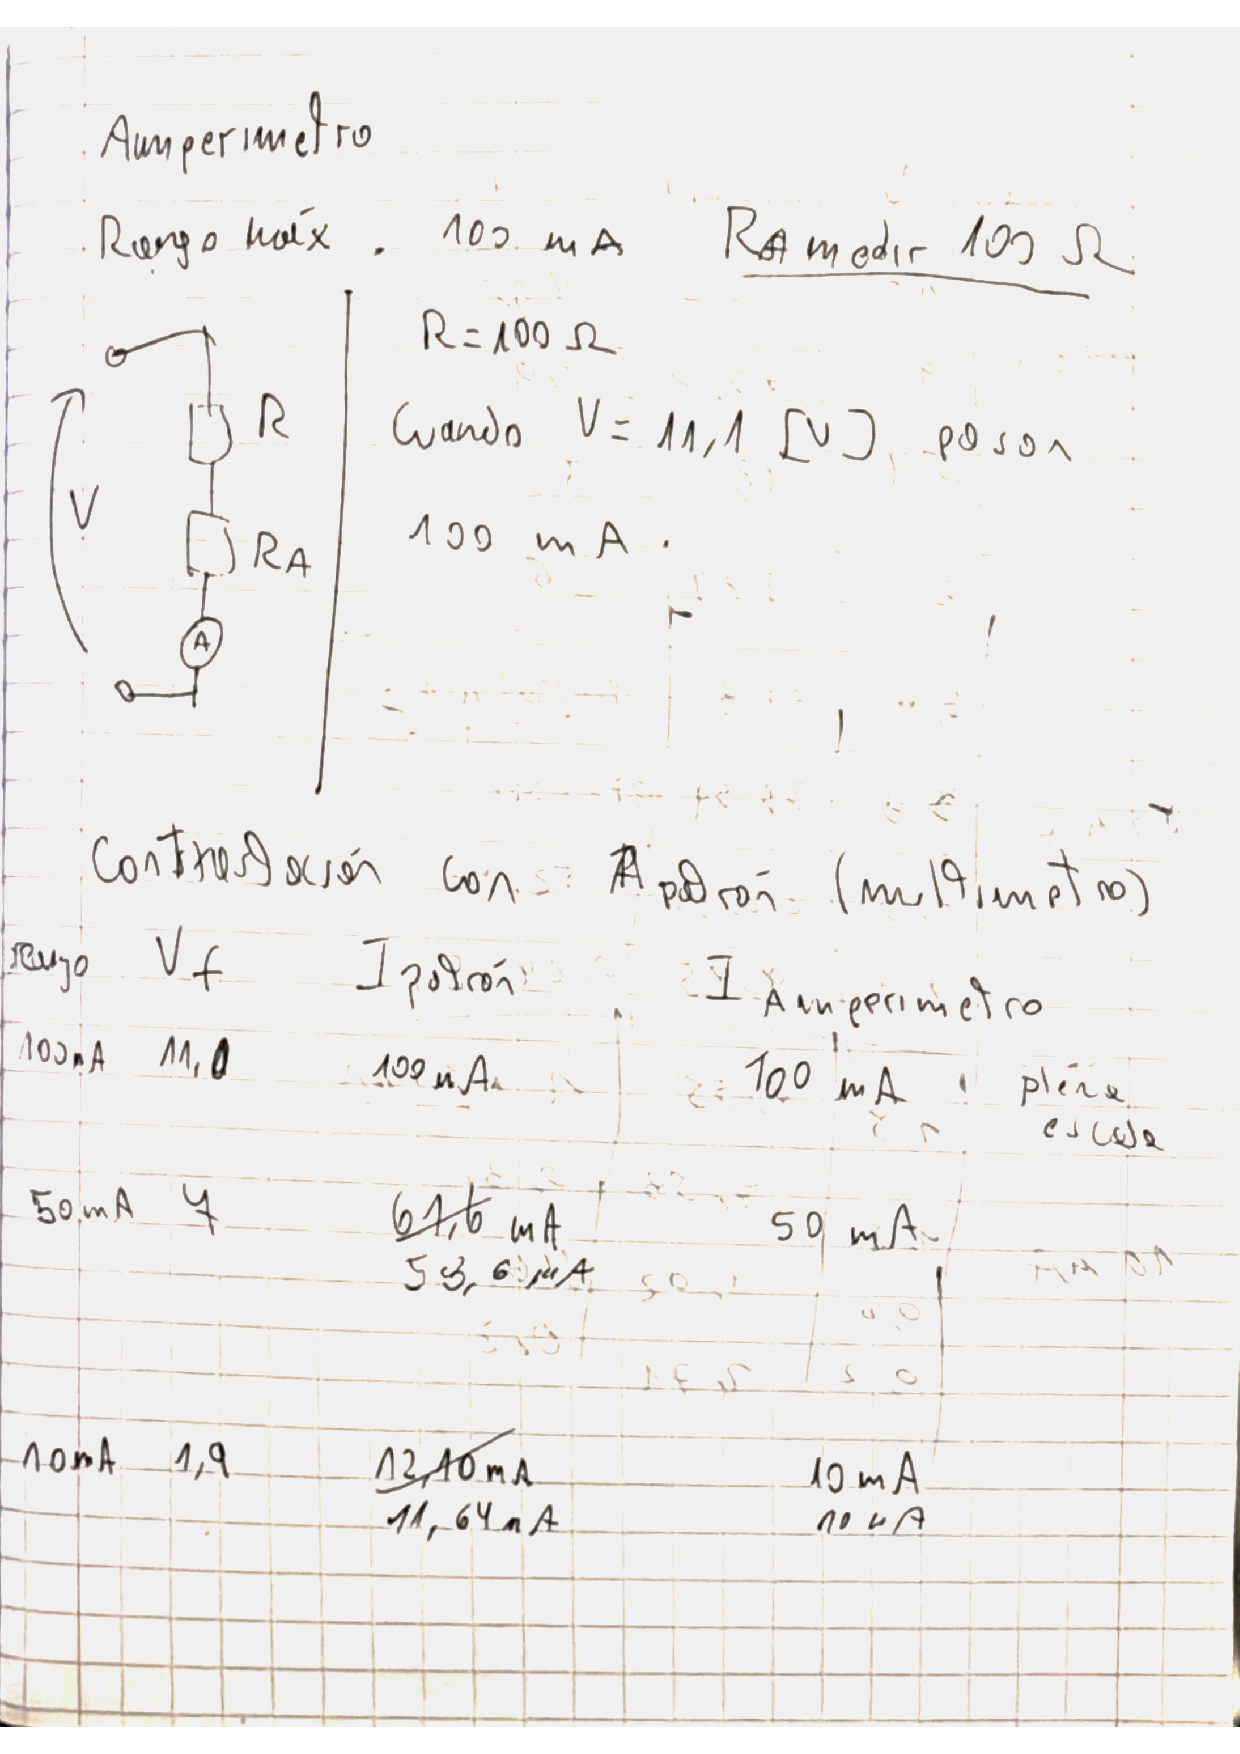
\includegraphics[width=0.8\linewidth]{recursos/10_1.pdf}
    \caption{Registro de los cálculos y contraste inicial del amperímetro analógico.
Se determinó la corriente total de 100 mA para el rango máximo con una resistencia limitadora de 100 $\Omega$.
Se observa el ajuste de la corriente del galvanómetro (Ig = 1 mA) y la corriente de prueba ($I_p$ = 100 mA) mediante la variación de $R_c$.
Además, se incluye la comparación con el amperímetro patrón (multímetro) para verificar la correspondencia de plena escala y los puntos intermedios de calibración.}
    \label{fig:placeholder}
\end{figure}


\begin{figure}[H]
    \centering
    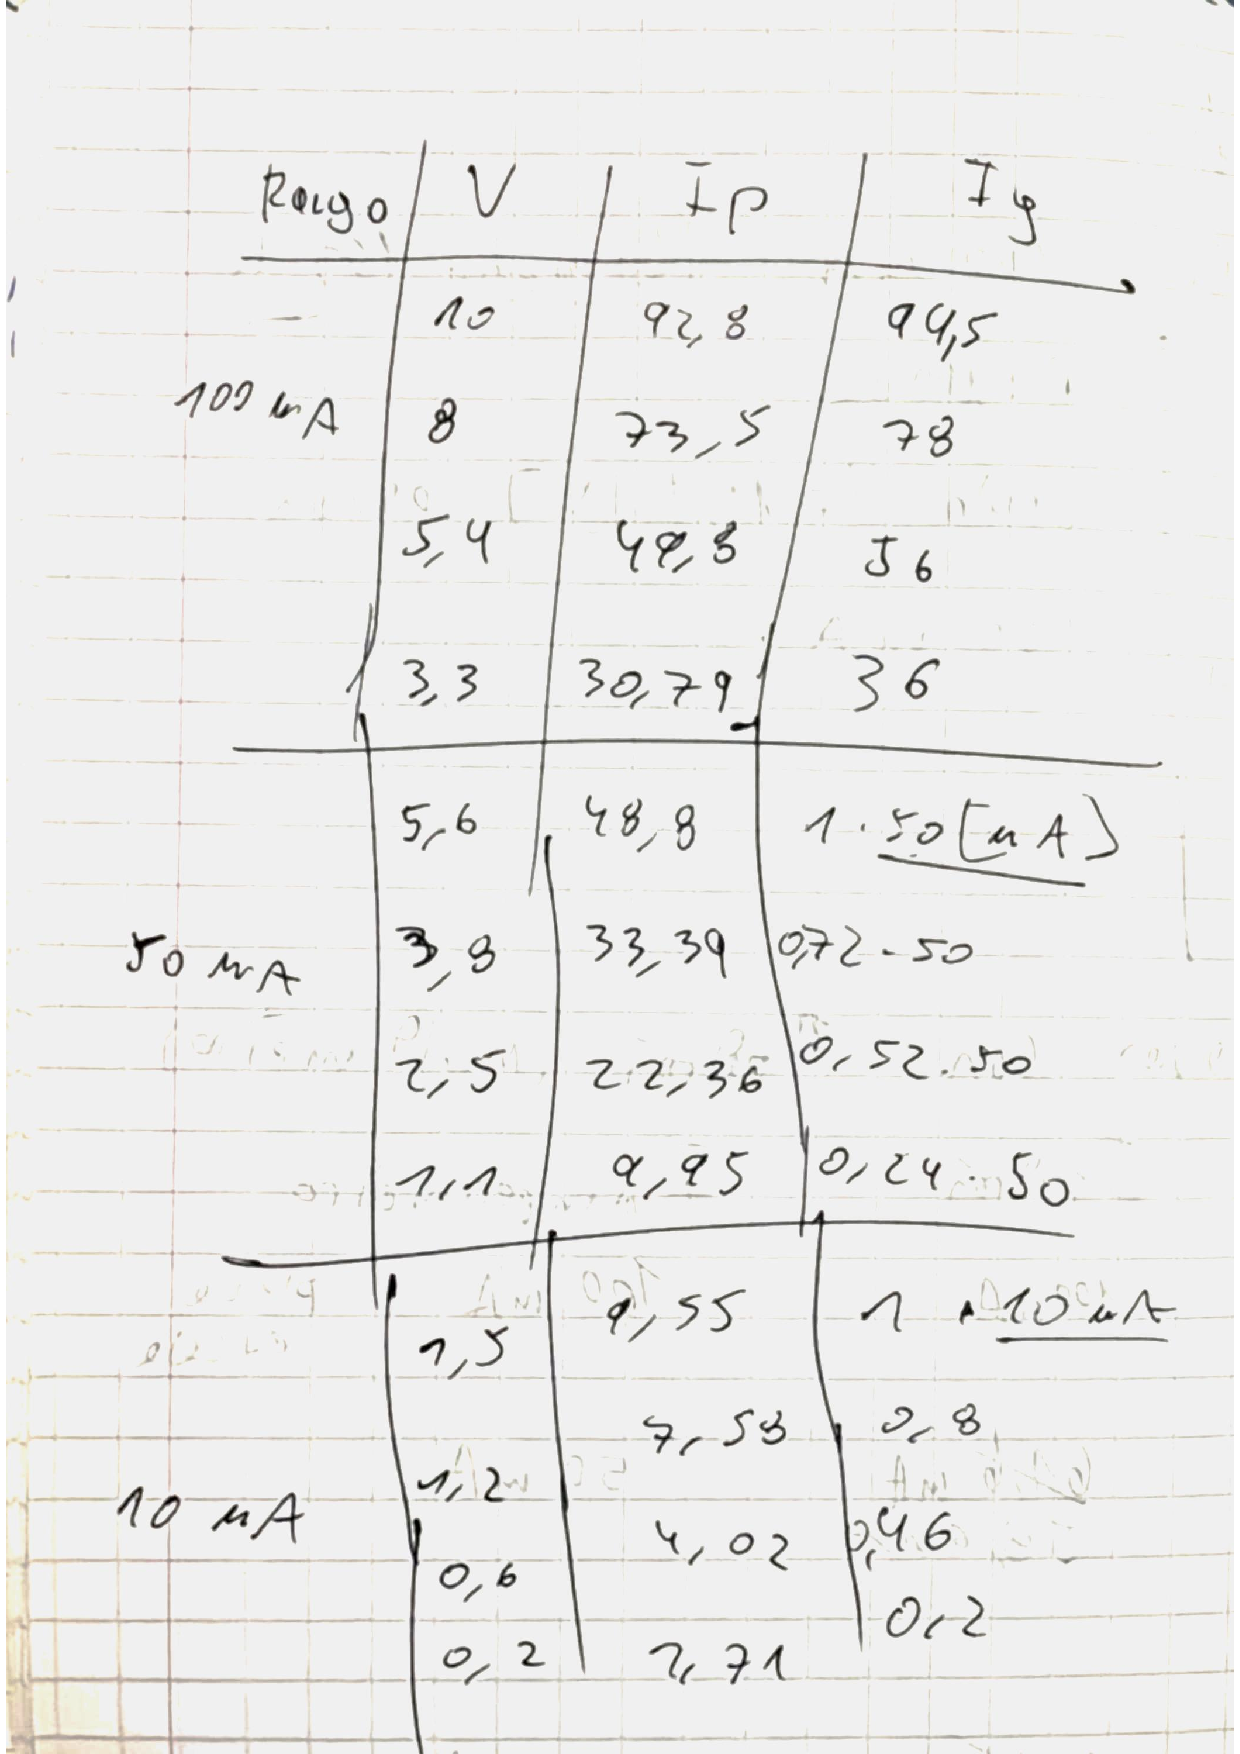
\includegraphics[width=0.8\linewidth]{recursos/10_2.pdf}
    \caption{Tabla de datos experimentales obtenidos en la verificación de la linealidad del amperímetro analógico.
Se registran los valores de tensión aplicada $V$, corriente patrón $I_p$ y corriente indicada por el galvanómetro $I_g$ en los tres rangos de medida: 100 mA, 50 mA y 10 mA.
Estos datos fueron utilizados para graficar la curva de linealidad y calcular el error porcentual de medición.}
    \label{fig:placeholder}
\end{figure}

\begin{figure}[H]
    \centering
    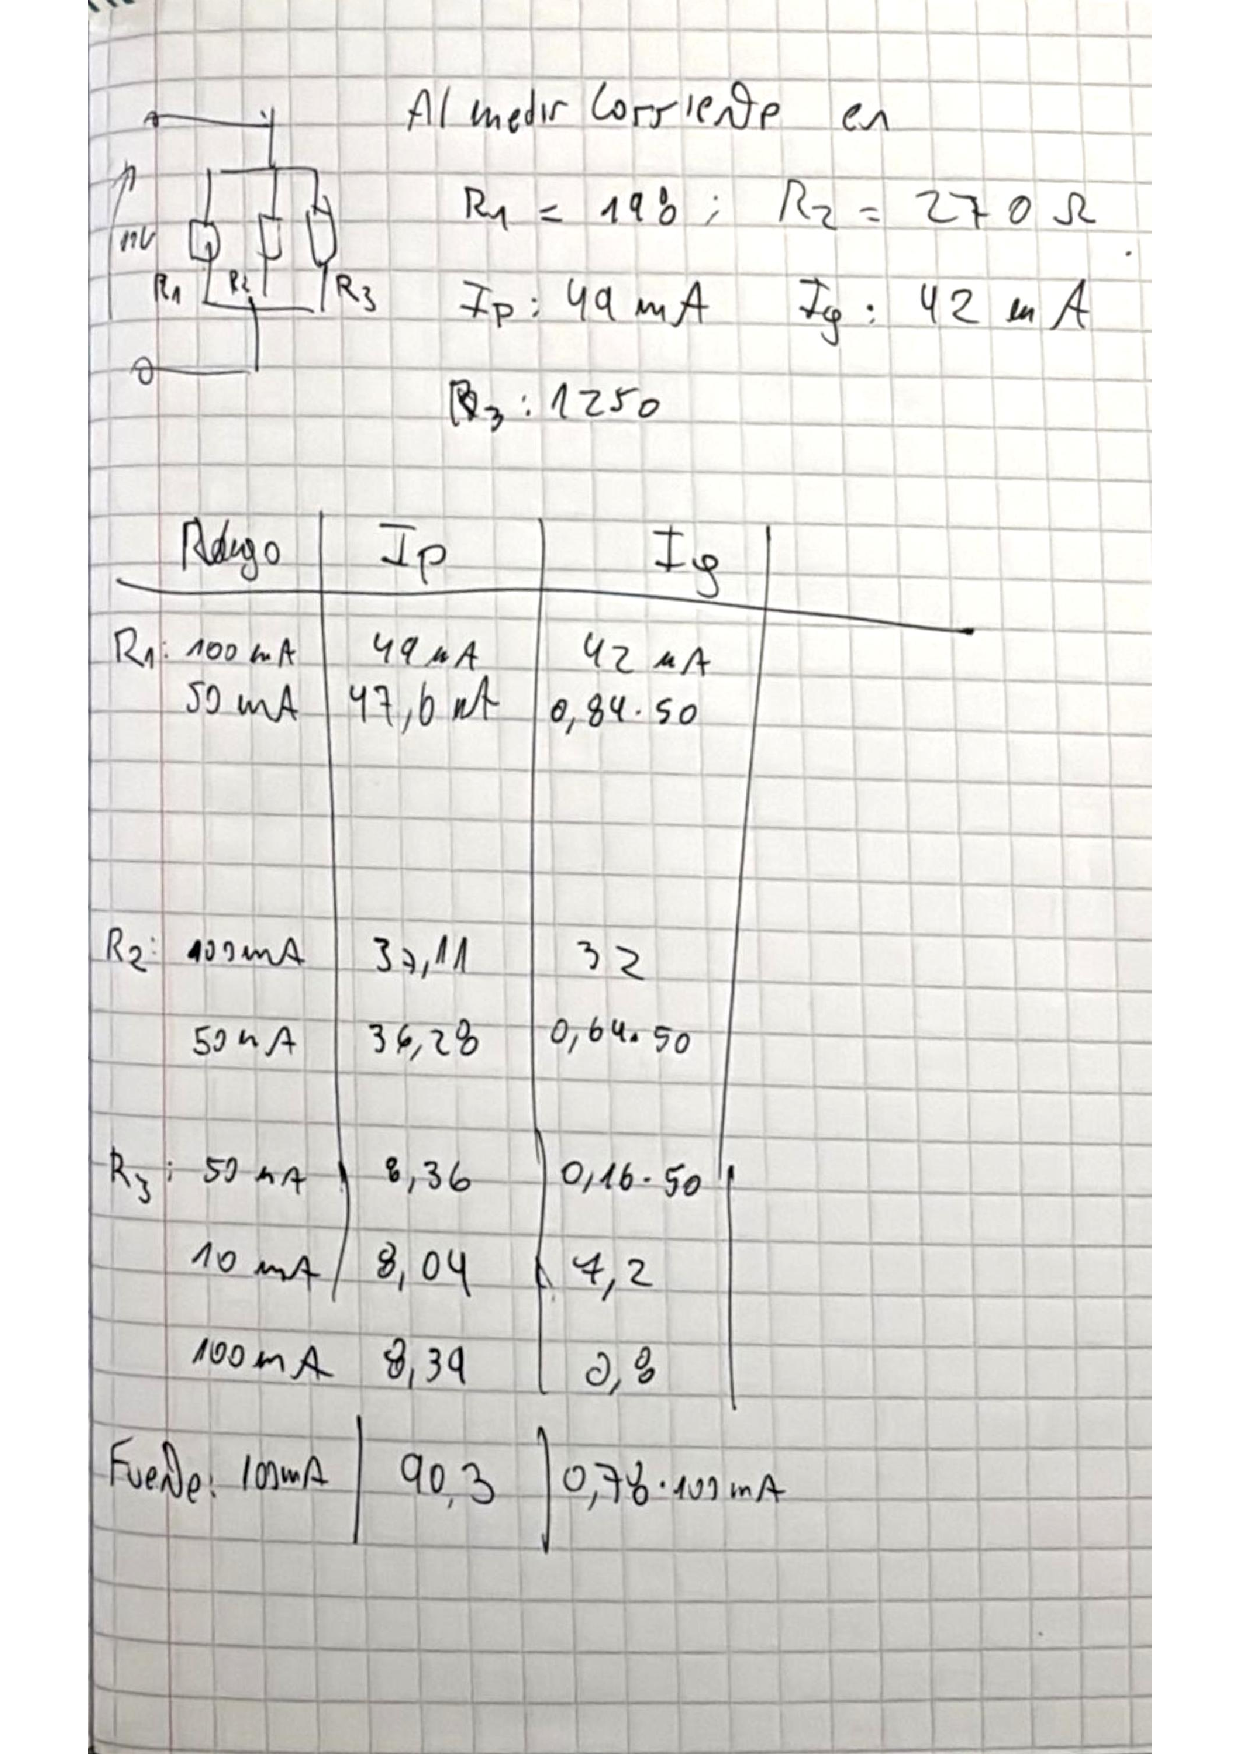
\includegraphics[width=0.8\linewidth]{recursos/10_3.pdf}
    \caption{Ensayo de medición de corrientes individuales y totales con resistores en paralelo.
Se utilizó una configuración con resistores de valores $R_1 = 198\, \Omega$, $R_2 = 270\ \Omega$, $R_3 = 125 \Omega$ aplicando una tensión de 10 $V_{cc}$.
Se compararon las corrientes medidas por el amperímetro $I_g$ con la corriente patrón $I_p$ en distintos rangos.
Este experimento permitió evaluar el error sistemático del instrumento y su comportamiento ante corrientes combinadas.}
    \label{fig:placeholder}
\end{figure}

\begin{figure}[H]
    \centering
    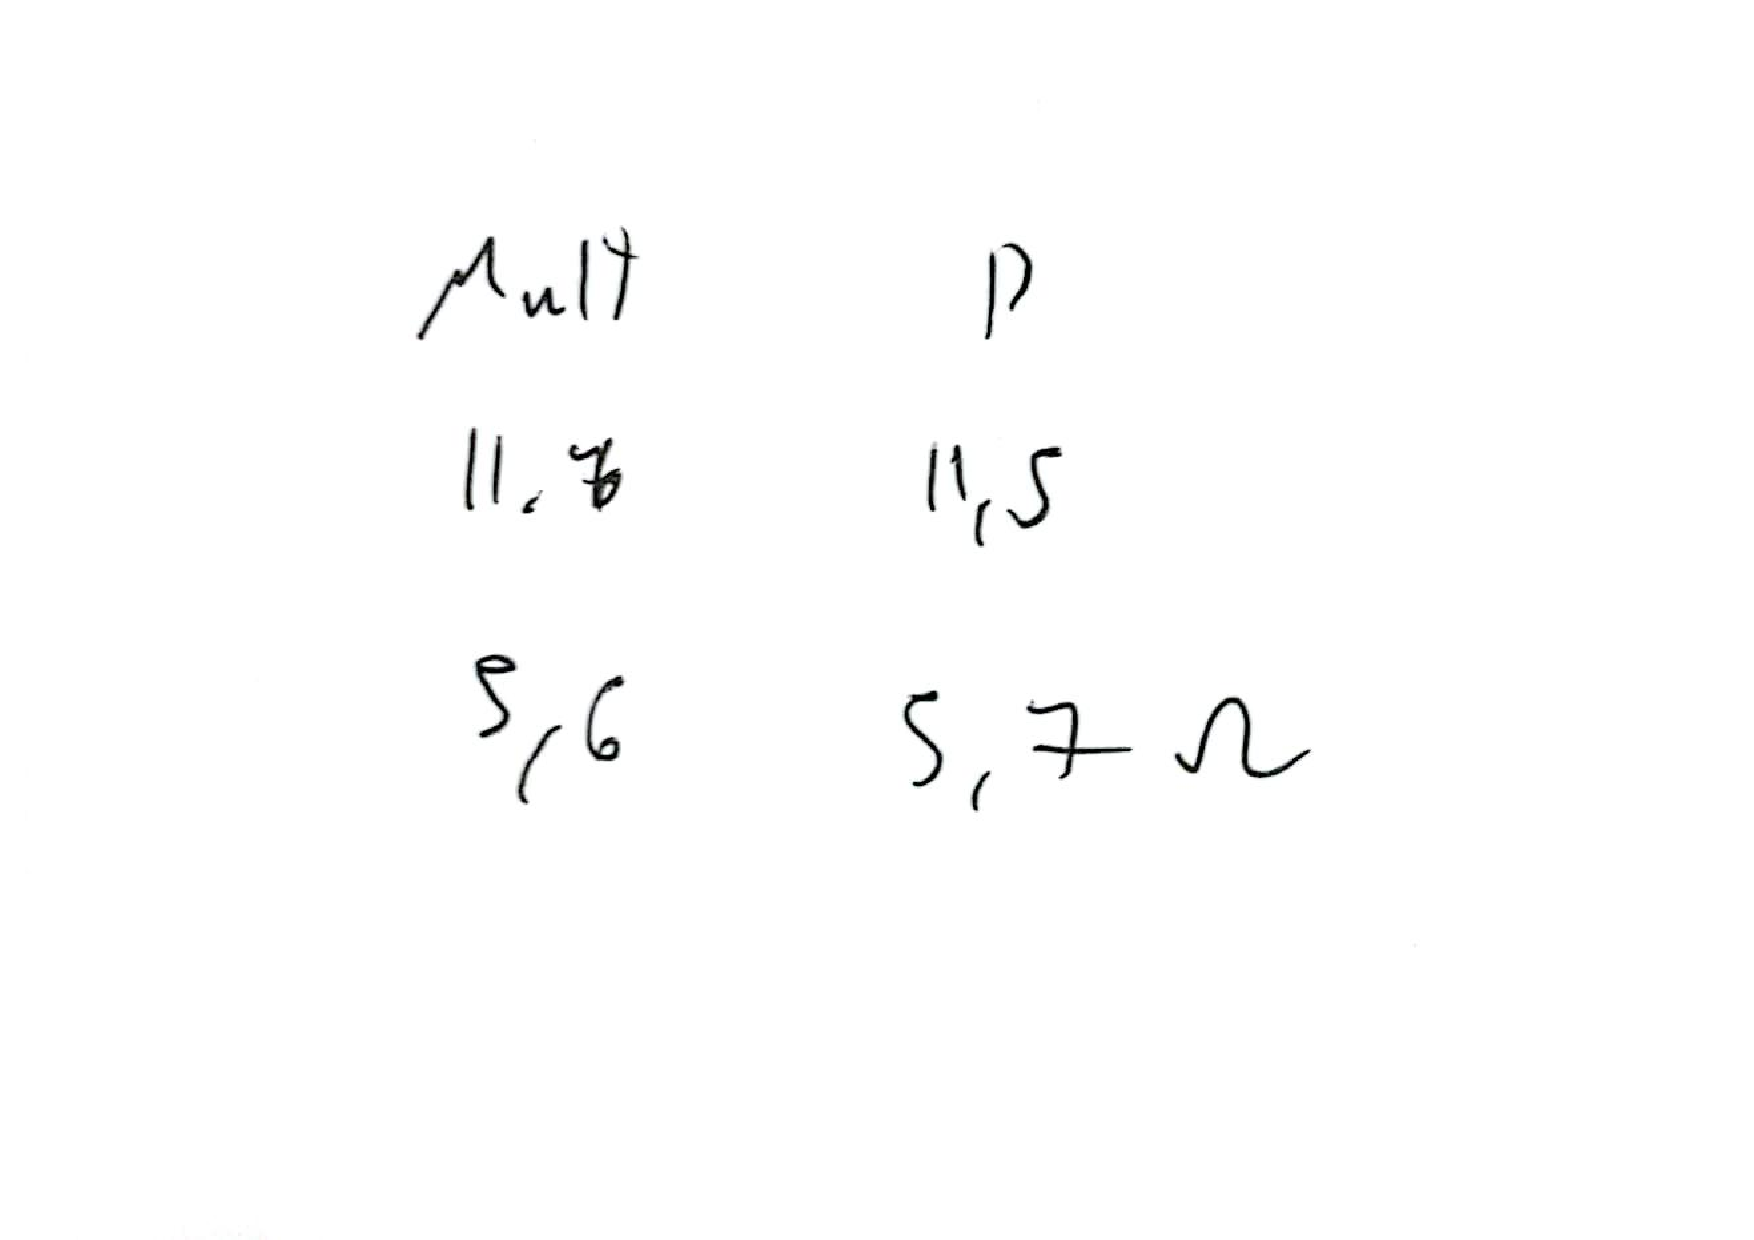
\includegraphics[width=0.75\linewidth]{recursos/10_4.pdf}
    \caption{En esta figura se presentan los resultados del contraste de las resistencias $R_{sh2}$ y $R_{sh3}$ utilizadas en el amperímetro analógico, medidas por dos métodos: con multímetro digital (columna “Mult”) y mediante el Puente de Kelvin (columna “P”).}
    \label{fig:placeholder}
\end{figure}